\documentclass{ifacconf}

\usepackage{natbib}            % you should have natbib.sty
\usepackage{graphicx}          % Include this line if your 
\usepackage{todo}
\usepackage{subfigure}

                               % document contains figures,
%\usepackage[dvips]{epsfig}    % or this line, depending on which
                               % you prefer.													
% predefined environments
%\begin{thm} ... \end{thm}		% Theorem
%\begin{lem} ... \end{lem}		% Lemma
%\begin{claim} ... \end{claim}	% Claim
%\begin{conj} ... \end{conj}	% Conjecture
%\begin{cor} ... \end{cor}		% Corollary
%\begin{fact} ... \end{fact}	% Fact
%\begin{hypo} ... \end{hypo}	% Hypothesis
%\begin{prop} ... \end{prop}	% Proposition
%\begin{crit} ... \end{crit}	% Criterion

\begin{document}

\begin{frontmatter}

\title{Scaling Communication of Energy Demand Flexibility using Destributed Aggregation} % Title, preferably not more than 10 words.

\thanks[footnoteinfo]{This articel is written as a part of the course Publishing Papers in the Peer-Reviewing System. It is based on \cite{} which is authored by Alex B. Andersen, Rasmus V. Prentow, and myself.}

\author[First]{Kim A. Jakobsen} 


\address[First]{Department of Computer Science, Aalborg University, Selma Lagerl\"{o}fs Vej 300 DK-9220 Aalborg East (e-mail: kjakob09@student.aau.dk).}                                              


          



\begin{abstract}                          % Abstract of not more than 250 words.
The system MIRABEL allows 
\end{abstract}

\end{frontmatter}

\section{Introduction}

\todo{aggregator = aggregator node}
\todo{BRP = BRP node}


Renewerable energy sources such as solar and wind share the undesirable attribute that they are uncontrollable. 
This is in contrast to e.g. fossile-fuled power plants where it is possible to ajust and control power production. 
Micro-Request-Based Aggregation, Forcasting and Scheaduling of Energy Demand, Supply and Distribution~\cite{} (MIRABEL) is a EU project that works to allow better unilization of renewerable energy. 
Insted of controlling the power production the goal is to predict and control the power consumption. 
If the Balance Responsible Party (BRP) can control when consumers use power and can forcast when renewerable energy is produced then it is only nessary to relay on fossile-fuel when renewerable energy is sparce.
The MIRABEL system allows consumers and producsers (prosumers) of energy to sent an offer of flexibility to the BRP, this is called a flex-offer. 
The BRP is now able to utalize more renewerable energy by shifting when energy is consumed.


An exempel of a flex-offer could be the heating of a swimmingpool. 
The consumer want his pool heated to 27$^\circ$ Celsius the next morning at 0700AM.
The swimmingpool heater sents a flex-offer to the local BRP containing the relevant information such as energy required and the timespan in which the heating can commence.
When the BRP recieve the flex-offer it is aggregated with other similar flex-offers. 
The aggregated flex-offer which now corresponds to a larger energy amount can now be shiftet to when there are renewerable energy available, this is also done by the BRP.  
The pool heater is informed when it should run and the consumer recives a discount on the energy price. 


MIRABEL have a large codebase which functions at a proof of concept level, one of the shortcommings in the project is the expensive communication.
The system simulates prosumers which sent flex-offers to a simulated BRP. 
This means that there is a many to one relationship between the prosumers and the BRP, this can be seen in Figure~\ref{fig:prosumerBrp}.
By introducing new intermediate nodes, it recieve flexoffers from the prosumer, aggregates them, and send the aggregated flex-offers to the BRP, we can distrubute the flex-offer load on these and reduce the message load on the BRP node. 
This new node type is called a aggregator node and can be seen in Figure~\ref{fig:prosumer-agg-brp}.

\begin{figure*}[]
   \centering
    \subfigure[Without aggregator nodes.]{
    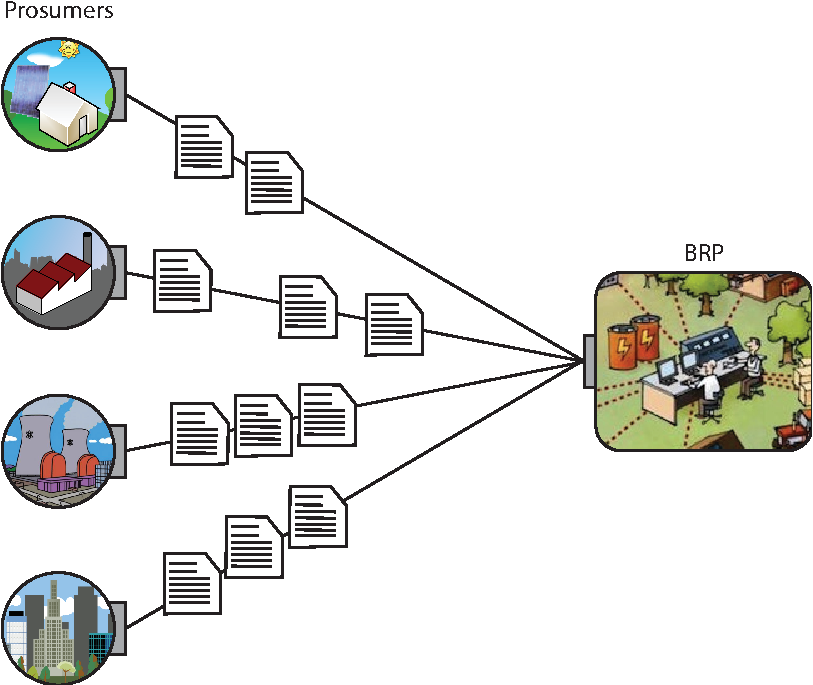
\includegraphics[width=0.75\columnwidth]{images/prosumer-brp.pdf}
    \label{fig:prosumerBrp}
   }
   \subfigure[With aggregator nodes.]{
    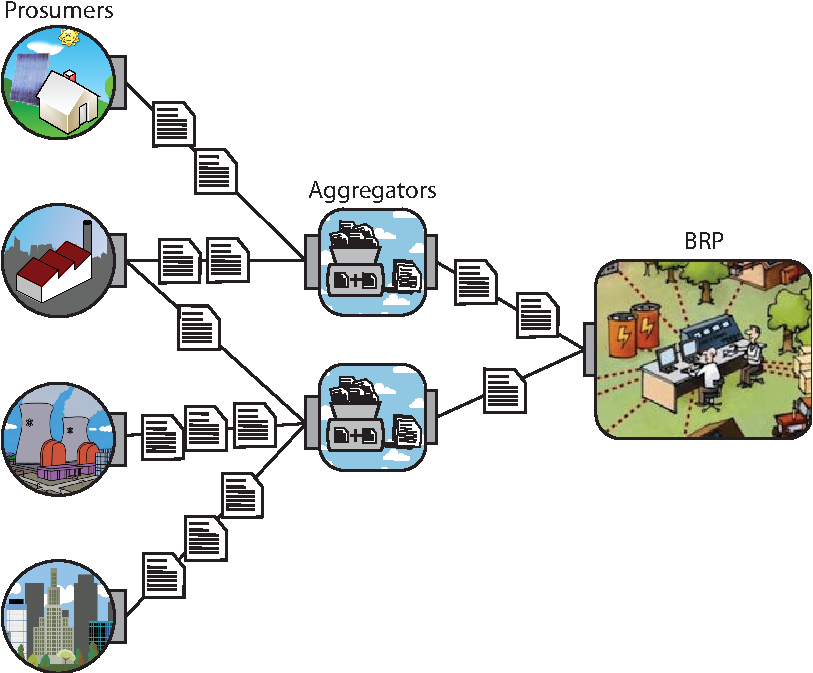
\includegraphics[width=0.75\columnwidth]{images/prosumer-agg-brp.pdf}
    \label{fig:prosumer-agg-brp}
   }  
  \caption{Four prosumers, displayed to the left of each sub-figure, sending flex-offers to a single BRP, displayed to the right.}
  \label{fig:communicationservice}
\end{figure*}


%nodes in mirabel
%report of what happens in the rest of the document

\section{related work}

In \cite{carmeli} they explore aggregation on sending side, network switches, and intermediate message servers.
The message server setup is similar to our approach but they assume that all messages can be aggregatet which is in contrast to this case.

Aggregation of flex-object which is a generalization of flex-offers, is explored and efficient algorithm are proposed in \cite{ssdbm}. 
These algorithm are implemented in the existing MIRABEL aggregation machanics which we reuse.

\section{Aggregator Node}

We now know that there is a number of prosumers that sent flex-offers to aggregator nodes. 
The flex-offers are aggregated info a few aggregated flex-offers and send to the BRP node.
To make it possible to compare different setups e.g. different number of aggregator nodes used, we define define a strategy.

Formally we describe a strategy that consists of four elements:
\begin{itemize}
	\item An aggregation function, it defines how the possible merging of flex-offers is done.
	\item A distribution function that defines how the flex-offers is allocated to the different aggregator nodes.
	\item A set of aggregator nodes.
	\item A BRP node.
\end{itemize} 


The naive approach is to make a strategy that have one aggregator node. 
This aggregator recieves all flex-offers and therefore have the best conditions for aggregating the flex-offers into as few as possible aggregated flex-offers. 
This would course the number of flex-offers send to the BRP node to be as the lowest possible. 
However, this would only move the scalability problem to the aggregator node insted of the BRP node. 

To express the desired effects of a stretegy we define the expression load.
Load on a given node is defined by the number of flex-offers it recieves.
It is desirable to have a stretegy renders as low as possible load on the BRP node and it is also desirable that the maximum load of the set of aggregators is low as possible.  


We propose the Evenly Distributing Strategy.
This strategy is defined as following:
\begin{itemize}
	\item As aggregation function we use the proposed algoithm described in \cite{ssdbm}.
	\item As distribution function we use a round-robin algorithm which distribute the flex-offers evenly amongst the aggregator nodes.
	\item We use a differnt number of aggregators for different experiments.
	\item A brp is used.
\end{itemize}

\section{Experimental Evaluation}
\subsection{Experimental Data}

The data used in this project is from the MeRegio project~\cite{meregio}. 
We only use consumption data in this experiment because we deem that it is not necessary generate production flex-offers to achieve realistic data.  
All the tests are run in accelerated time.


We test six strategies that only vary on the set of aggregates. The test is conducted with 0, 1, 2, 4, 8, and 16 aggregators. 
To test if the aggregator node reduces the amount of flex-offers received by the BRP we run the experiment with an average of 100, 1000, and 10,000 flex-offers send per time unit. 

\subsection{Results}
\todo{brug load mere}

\begin{figure*}[]
   \centering
    \subfigure[Without aggregator nodes.]{
    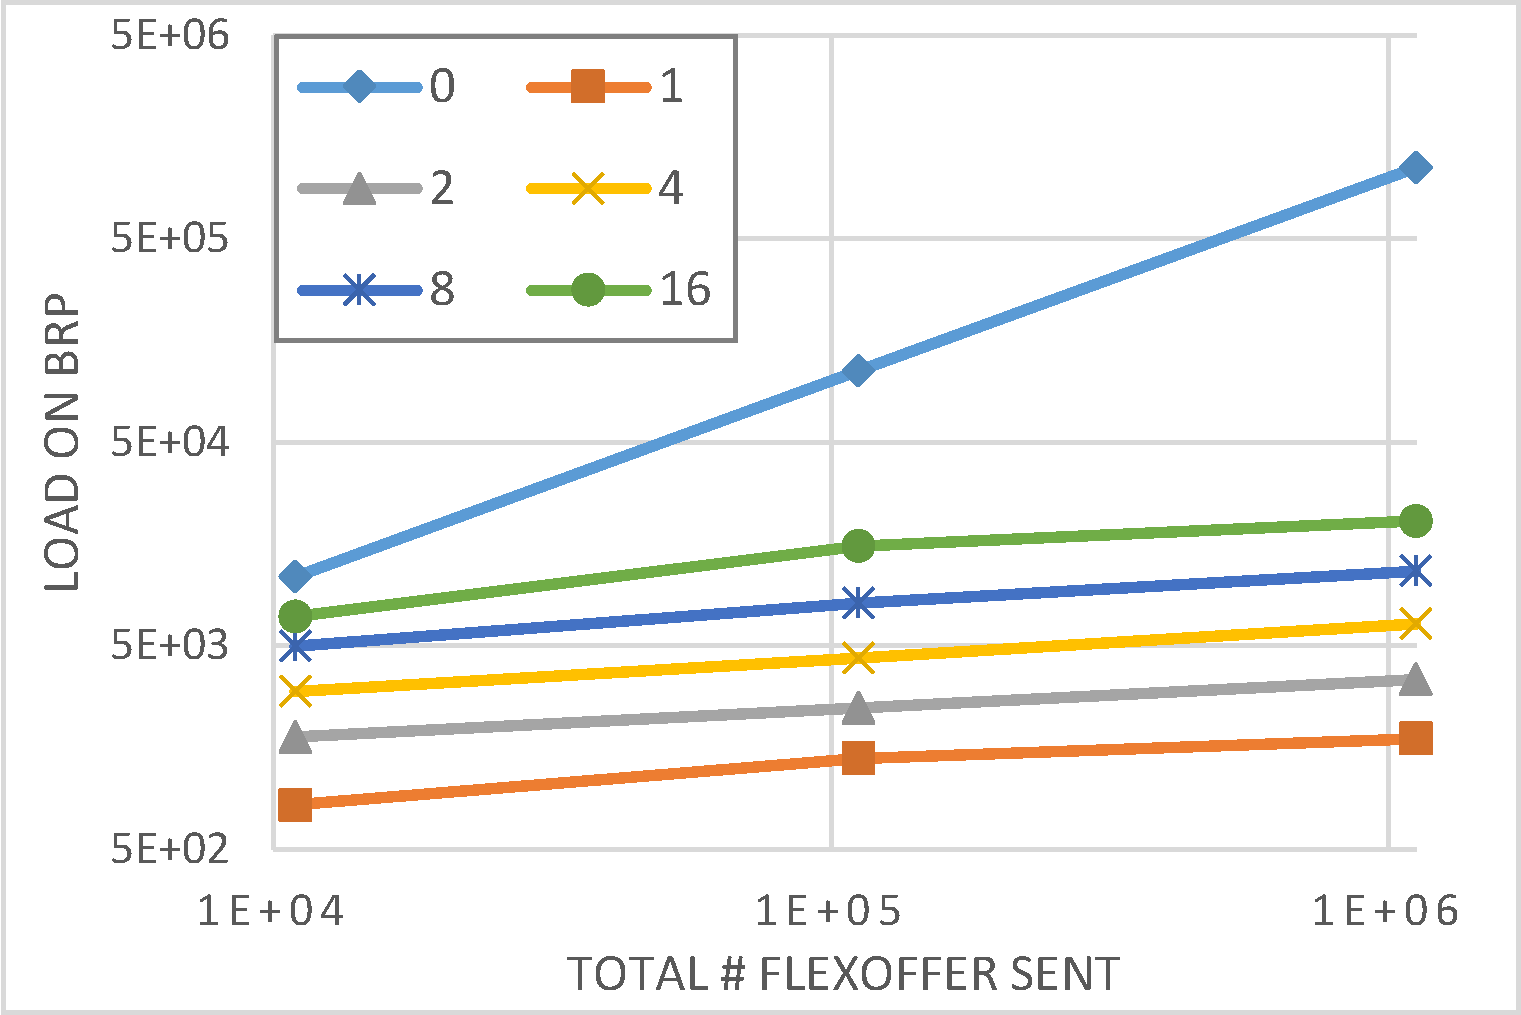
\includegraphics[width=0.75\columnwidth]{images/resultA.pdf}
    \label{fig:prosumerBrp}
   }
   \subfigure[With aggregator nodes.]{
    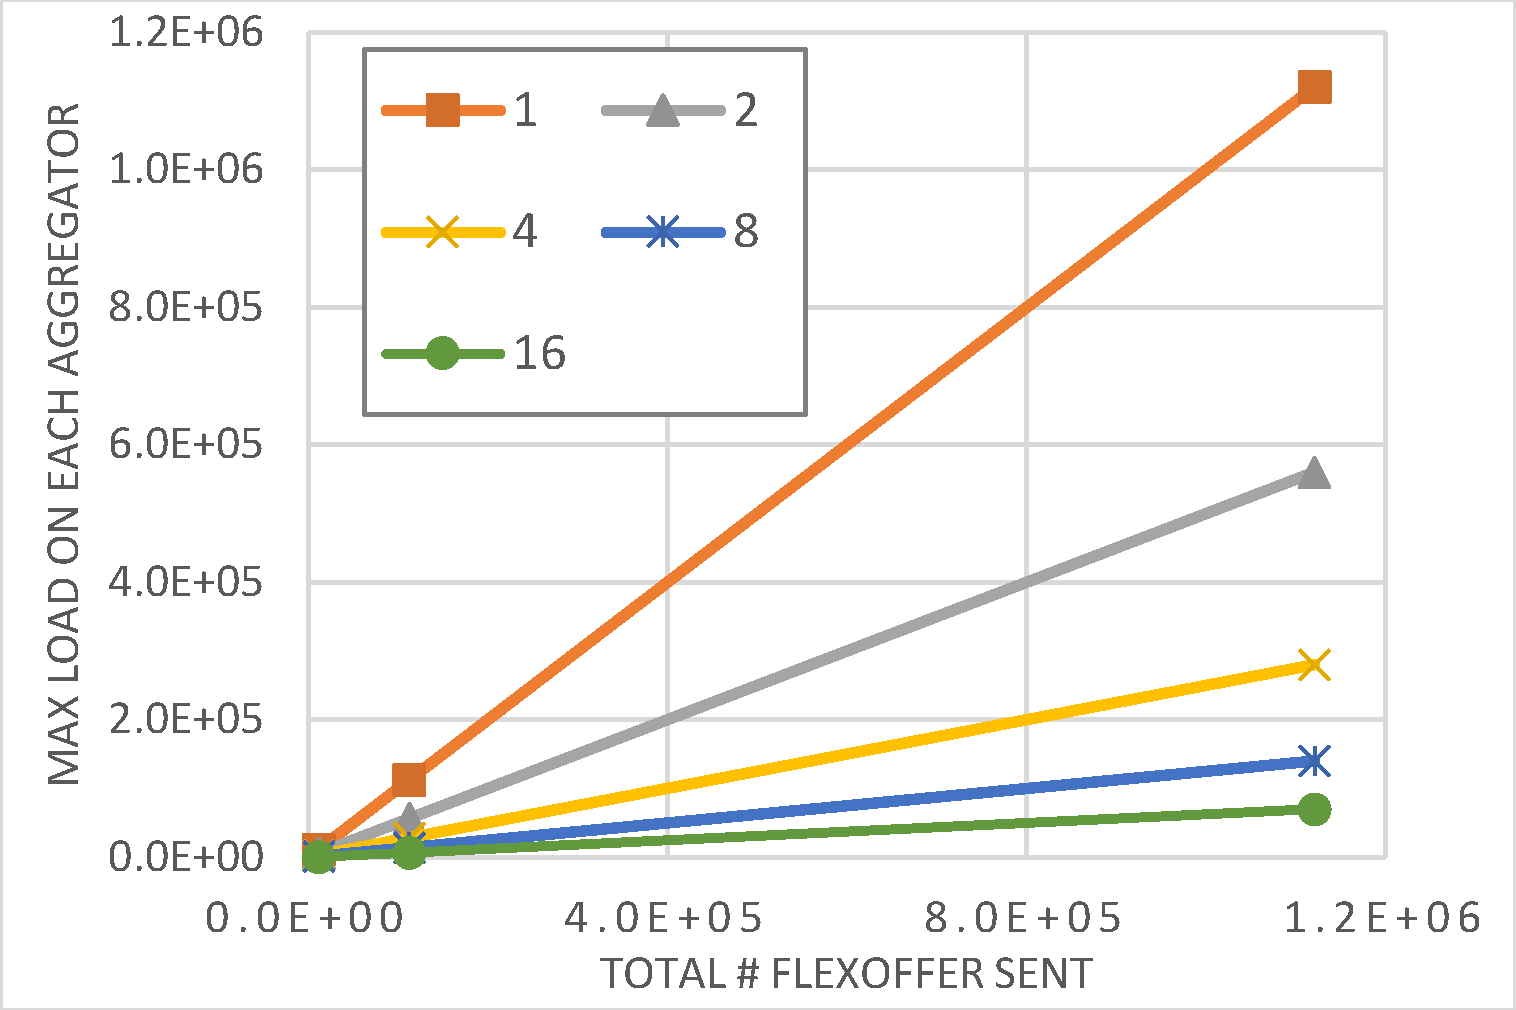
\includegraphics[width=0.75\columnwidth]{images/resultC.pdf}
    \label{fig:prosumer-agg-brp}
   }  
  \caption{Four prosumers, displayed to the left of each sub-figure, sending flex-offers to a single BRP, displayed to the right.}
  \label{fig:communicationservice}
\end{figure*}

\begin{figure}%
\centering
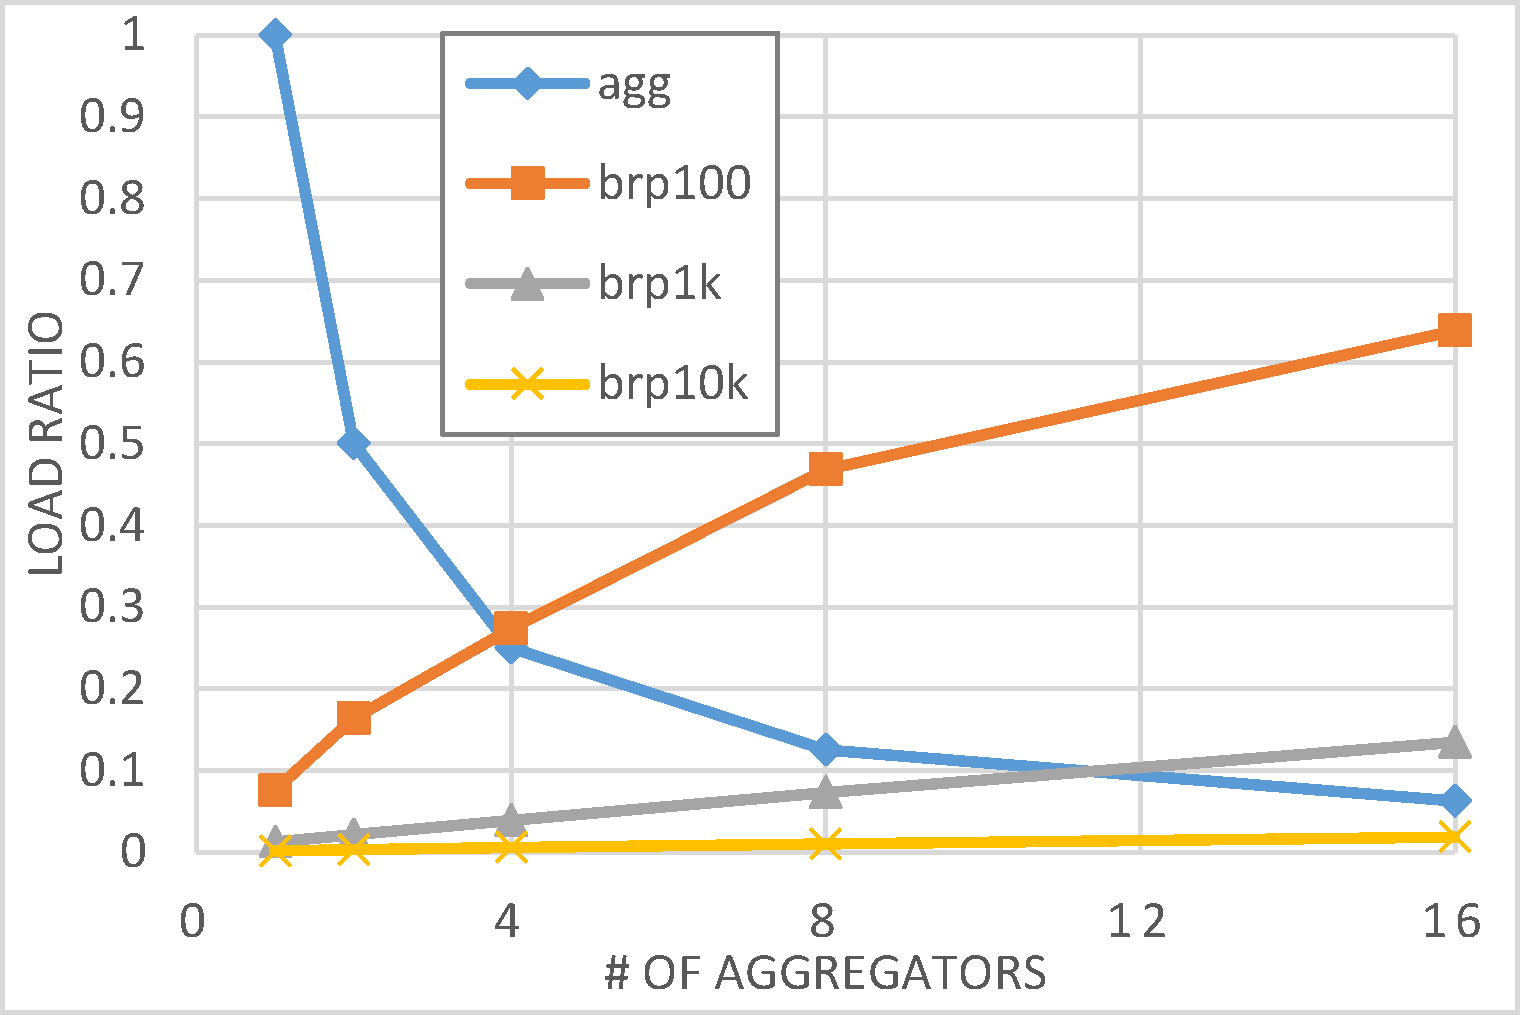
\includegraphics[width=0.75\columnwidth]{images/resultD.pdf}
\caption{}%
\label{}%
\end{figure}



In Figure \ref{fig:brpload} the load on the BRP is shown in a double logarithmic graph. 
The legend shows the number of aggregators corresponding to the six different stretegies, 
the x-axis is the total number of flex-offers sent, 
and the y-axis shows the total number of flex-offers the BRP recieves.

In Figure \ref{fig:aggload} the load on the aggregator\(s\) is shown. 
The x-axis is the total number of flex-offers sent,
and the y-axis is the maximum number of flex-offers recieved by the set of aggregators used. 
Remember that all the stretegies use round-robin algorithm as distribution function. 

The results indikate that load on the BRP is lower if only one aggregator is used. 
This is because when the flex-offers are spred across more aggregator nodes the aggregator node will not be able to aggregate as many flex-offers as if one single aggregator node had all the flex-offers. 
This means that if one aggregator node recieve all the flex-offers then is able to reduce the number of flex-offers sent to the BRP.

We assume that it is desirable that the number of flexoffers recieved by both the aggregator nodes and the BRP is kept as low as possible.
It is then possible to combine the two graphs and find the intersections.
The intersections represents the optimal number of aggregator nodes at the given number of flex-offers. 

In Figure \ref{fig:intersection} the load of the aggregators and the load of the BRP is displayed.
The x-axis is the number of aggregators, and the y-axis is a presentage representation of the load on the nodes.
The blue line line represents load on the aggregator node.
The red, gray, and blue are the load on the BRP node with respectivly with an average of 100, 1000, and 10,000 flex-offers send per time unit.

The two visible intersectoins indicate the optimal set of aggregaters at an given average of flex-offers sent. 
These results allows us to determine the number of aggregator nodes to use when the average number of flex-offers sent is know, and our proposed strategy is used.   

\section{Conclusion and future work}

%the number of flexoffers may vary, = make number of aggregator nodes dynamic.


%important to balan






\appendix
\bibliography{bibtex/bib}{}
\end{document}